\subsection{Diseño}

En la figura \ref{diseño} se presenta el esquemático completo del circuito implementado para este proyecto.

Con respecto a la pantalla LCD solo se trató de conectar los pines necesarios por la pantalla para cumplir con los requerimientos de lo que se desea imprimir; esto fue más seguir la conexión en base al firmware, que diseño de electrónica como tal. Esta pantalla, según las especificaciones técnicas, presenta un consumo de $0.125\textit{mV}$.

Seguidamente, el consumo más significativo será por parte del bombillo; el cual, según las especificaciones técnicas tiene un consumo de $60 \textit{Watts}$. Tanto el dimmer, como el relé, tienen una caída de tensión no significativa; al igual que los cables por ser de poca longitud presentan una caída de tensión mínima con respecto al consumo principal. Por lo que el consumo total se podría reducir al bombillo. En base a este consumo se diseña. \\
El relé puede manejar corrientes de contacto de $[10, 250]A$ AC o $30V$DC, con un voltaje de bobina de  $12V$ por canal. Posee voltaje de operación, en conjunto de $[5, 12]V$, y maneja $[3, 5]V$ por cada canal.

\begin{figure}[H]
\centering
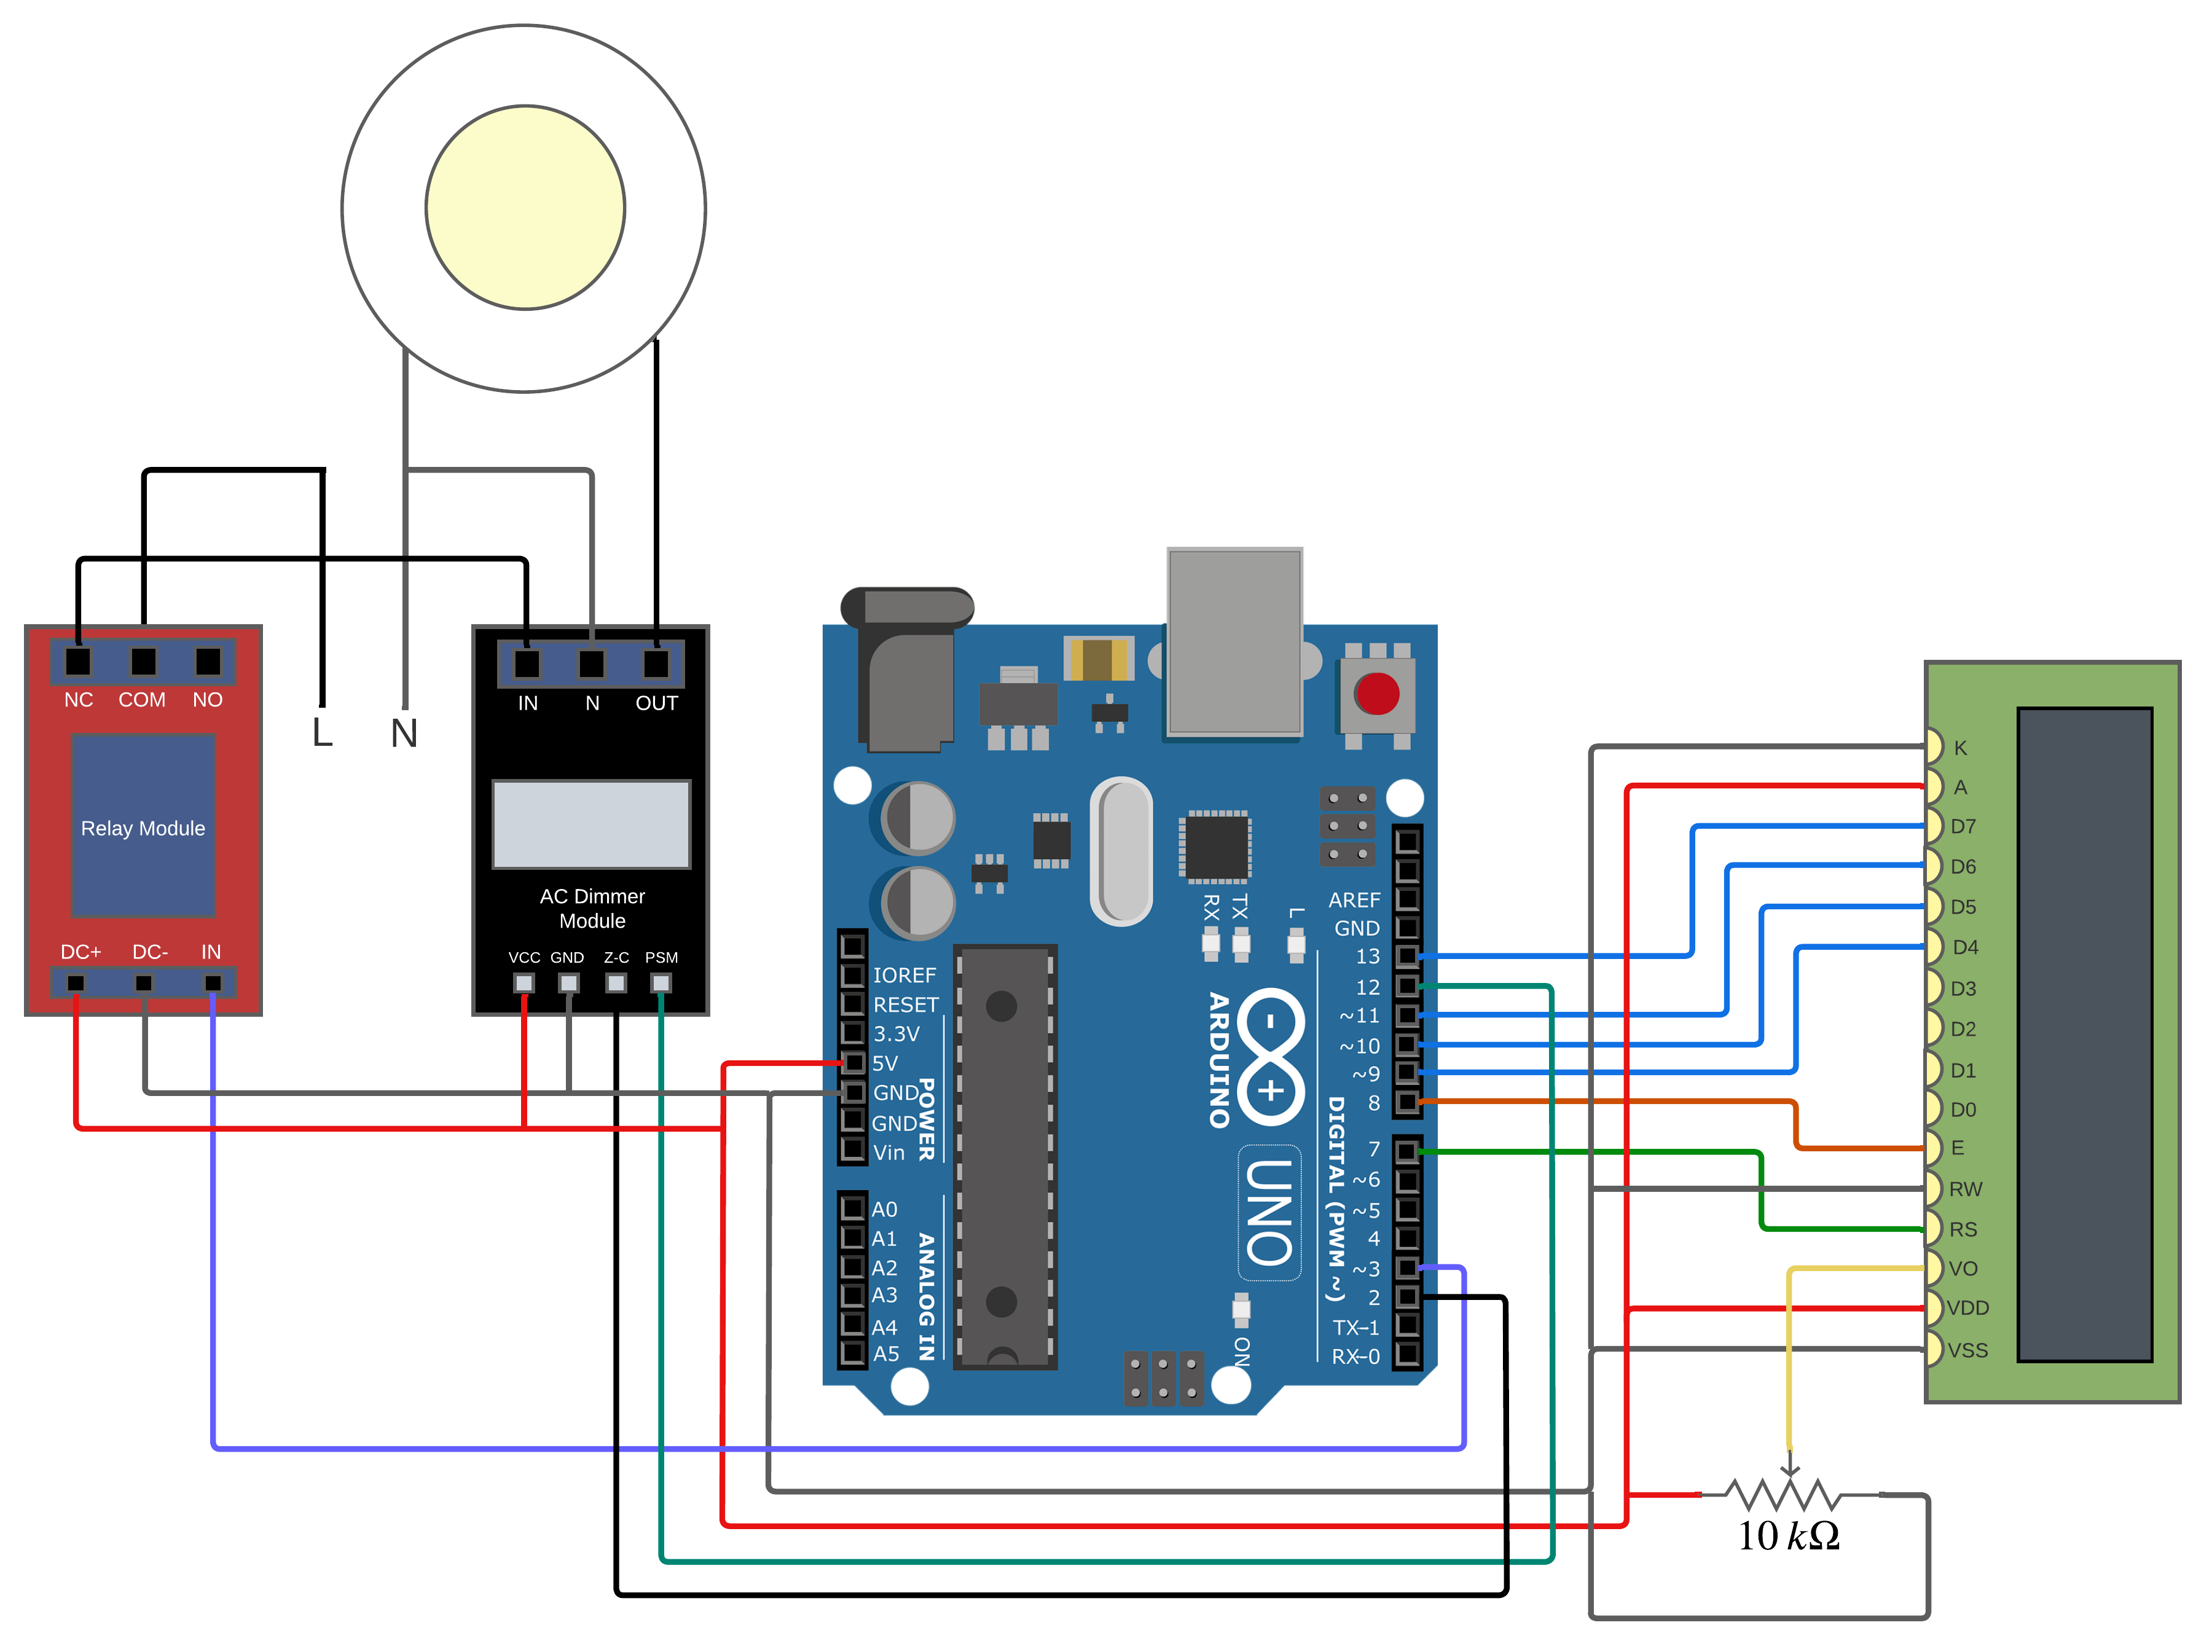
\includegraphics[scale=0.56]{./images/esquematico_completo.png} 
\caption{Esquemático a diseñado (Autoría propia).}
\label{diseño}
\end{figure}


